\documentclass[aspectratio=169, 11pt]{beamer}
\usepackage[utf8]{inputenc}
\usepackage[spanish]{babel}
\usepackage{amsmath,amsfonts,amsthm,amssymb,mathtools,sectsty}
\pagenumbering{gobble}
\usepackage{subcaption}
%\usepackage{graphicx}
%\usepackage[pdftex,dvipsnames]{xcolor}
\usepackage{cancel}
\usepackage{graphicx}
\usepackage{marginnote}
\usepackage{mathabx}
\usepackage{float}
\setlength{\marginparwidth}{2cm}

% Tikz y las librerías para automátas
\usepackage{tikz-cd}
\usepackage{tikz}
\usetikzlibrary{arrows,automata}
\usetikzlibrary{babel} %para evitar que se jodan los automatas de tikz
\usetikzlibrary{graphs} 
\usetikzlibrary{calc}
\usetikzlibrary{positioning}
%\usetikzlibrary{shapes.geometric}  % for [ellipse], [diamond], etc

%\usepackage[backend=biber,...]{biblatex} 

%Referencias; me gustaría que backref funcione pero no es importante tampoco.
\usepackage[pagebackref]{hyperref}
% Para modificar el estilo de las referencias
\hypersetup{
	colorlinks,
	linkcolor={astral},
	citecolor={red!70!black},
	urlcolor={red!80!black}
}
\definecolor{astral}{RGB}{46,116,181}
\colorlet{chulo}{blue!70!purple}
\colorlet{rojo}{purple!45!black}
\definecolor{carrotorange}{rgb}{0.93, 0.57, 0.13}
\definecolor{brightcerulean}{rgb}{0.11, 0.67, 0.84}
\definecolor{brightube}{rgb}{0.82, 0.62, 0.91}
\definecolor{cadmiumred}{rgb}{0.89, 0.0, 0.13}
\definecolor{applegreen}{rgb}{0.55, 0.71, 0.0}
\definecolor{aurometalsaurus}{rgb}{0.43, 0.5, 0.5}

%%%%%%%%%%%%%%%%%%%%% ENUMERAR CON COSAS QUE NO SEAN SOLO NÚMEROS %%%%%%%%%%
\usepackage[shortlabels]{enumitem}
\setlist[enumerate]{font=\bfseries}
\usepackage{adjustbox}


%%%%%%%%%%%%%%%%%%%%%%% TÍTULOS DE SECCIONES MÁS FANCIES %%%%%%%%%%%%%%
\usepackage{titlesec}
\setcounter{secnumdepth}{3} % Hasta que profundidad quiero numerar, 4 sería los párrafos.
\titleformat{\section}[block]{\color{astral!50!black}\Large\bfseries\filcenter}{\S\thesection.}{1em}{}
\titleformat{\subsection}[hang]{\color{astral!50!black}\large\bfseries\filcenter}{\S\thesubsection.}{1em}{}

%%%%%%%%%%%%%%%%%%%%%% COLORES PÁRRAFOS Y CAPÍTULOS %%%%%%%%%%%%%%%%%%%%%%%%
%\paragraphfont{\color{astral!70!black}}
\chapterfont{\color{astral!40!black}}
%\subsectionfont{\color{astral!60!black} }
%\sectionfont{\color{astral!50!black} }

\usepackage{mathpazo}
\usepackage{amssymb}
%\usepackage{thmtools}

%Esto sirve para armar grafos de Cayley de una manera más copada.
\usetikzlibrary{lindenmayersystems,arrows.meta}
\pgfdeclarelindenmayersystem{cayley}{
	\rule{G->G-G+++G--G}
	\symbol{R}{
		\pgflsystemstep=0.5\pgflsystemstep
	}

}

\usepackage[framemethod=tikz]{mdframed}

%%%%%%%%%%%%%  TEOREMAS  %%%%%%%%%%%%%%%%%
\theoremstyle{plain} %% el estilo clásico
\newtheorem{teo}{\color{rojo}{ { Teorema}}}[section]
\newtheorem{prop}[teo]{\color{rojo} {Proposición}}
\newtheorem{lema}[teo]{\color{rojo} {Lema}}
\newtheorem{coro}[teo]{\color{rojo} {Corolario}}
\newtheorem*{aff}{ {Afirmación}}
% Si pongo [theorem] siguen la numeración de los teoremas. 
% e.j. Teo 1, Lema 2, Teo 3, Teo 4 ...
\theoremstyle{definition}
\newtheorem{deff}[teo]{{ Definición}}{\smallskip}
\newtheorem{ej}[teo]{{Ejemplo}}{\smallskip}

% Remarks
\theoremstyle{remark}
\newtheorem{obs}[teo]{ {Observación}}{\smallskip}

%%%%%%%%%% FRAMES PARA TEOREMAS A LO HATCHER %%%%%%%%%%%%%%%%%%%%%%%%%

\surroundwithmdframed[outerlinewidth=0.4pt,
innerlinewidth=0.4pt,
align=center,
middlelinewidth=1pt,
middlelinecolor=white,
innertopmargin=-4pt,
innerbottommargin=0pt,
innerrightmargin=4pt,
innerleftmargin=4pt,
bottomline=false,topline=false,rightline=false]{teo}
\surroundwithmdframed[outerlinewidth=0.4pt,
innerlinewidth=0.4pt,
align=center,
middlelinewidth=1pt,
middlelinecolor=white,
innertopmargin=-4pt,
innerbottommargin=0pt,
innerrightmargin=4pt,
innerleftmargin=4pt,
bottomline=false,topline=false,rightline=false]{lema}

\surroundwithmdframed[outerlinewidth=0.4pt,
innerlinewidth=0.4pt,
align=center,
middlelinewidth=1pt,
middlelinecolor=white,
innertopmargin=-4pt,
innerbottommargin=0pt,
innerrightmargin=4pt,
innerleftmargin=4pt,
bottomline=false,topline=false,rightline=false]{prop}


\surroundwithmdframed[outerlinewidth=0.4pt,
innerlinewidth=0.4pt,
align=center,
middlelinewidth=1pt,
middlelinecolor=white,
innertopmargin=-4pt,
innerbottommargin=0pt,
innerrightmargin=4pt,
innerleftmargin=4pt,
bottomline=false,topline=false,rightline=false]{coro}

%==================================================================%

% DEMOS EN NEGRITA.
\renewenvironment{proof}{{\textbf{Demostración.}}}{ \hfill $\blacksquare$ \medskip} 

%% ========== Para escribir pseudo ==========
%\usepackage{algorithm}
%\usepackage[noend]{algpseudocode}  % "noend" es para no mostrar los endfor, endif
%%\algrenewcommand\alglinenumber[1]{\tiny #1:}  % Para que los numeros de linea del pseudo sean pequeños
%\renewcommand{\thealgorithm}{}  % Que no aparezca el numero luego de "Algorithm"
%\floatname{algorithm}{ }    % Entre {  } que quiero que aparezca en vez de "Algorithm"
%
%% traducciones
%\algrenewcommand\algorithmicwhile{\textbf{mientras}}
%\algrenewcommand\algorithmicdo{\textbf{hacer}}
%\algrenewcommand\algorithmicreturn{\textbf{devolver}}
%\algrenewcommand\algorithmicif{\textbf{si}}
%\algrenewcommand\algorithmicthen{\textbf{entonces}}
%\algrenewcommand\algorithmicfor{\textbf{para}}
%
%%% indentar dentro de los algoritmos
%\algdef{SE}[SUBALG]{Indent}{EndIndent}{}{\algorithmicend\ }%
%\algtext*{Indent}
%\algtext*{EndIndent}

% =========================================================
\usepackage[colorinlistoftodos,prependcaption,textsize=tiny]{todonotes}



%Comandos útiles.
\newcommand\RP{\mathbb{RP}}
\newcommand{\norm}[1]{\left\lVert#1\right\rVert}
\newcommand{\RR}{\mathbb{R}}
\newcommand{\CC}{\mathbb{C}}
\newcommand{\NN}{\mathbb{N}}
\newcommand{\ZZ}{\mathbb{Z}}
\newcommand{\Om}{\Omega}
\newcommand{\A}{\mathcal A}
\newcommand\ol{\overline}
\newcommand{\blue}{\textcolor{chulo}}
\newcommand{\red}{\textcolor{rojo}}
\newcommand{\Gg}{\mathfrak g}
\newcommand{\SL}{SL_2(\mathbb Z)}
\newcommand{\stab}{\text{Stab}}
\newcommand{\ic}{independiente de contexto }
\newcommand{\APND}{automáta de pila no determinístico }
\newcommand{\APD}{automáta de pila determinístico }
\newcommand{\gramatica}{{\cal G} = (V, \Sigma, P, S)}
\newcommand{\deriva}{\overset{*}{\to_{\cal G}}}
\newcommand{\tto}{\overset{*}{\to}}
\newcommand{\lengderivado}{L({\cal G})}
\newcommand{\fg}{grupo finitamente generado }
%\newcommand{\ol}{\overline{}}
\newcommand{\aut}{\text{Aut}}
\newcommand{\Sy}{\text{Sym}} 

\newcommand{\cay}[2]{\text{Cay}(#1,#2)}

\newcommand{\partes}[1]{{\cal{P}}(#1)} 

\newcommand*{\deri}{{\cal D}}
\newcommand*{\lexorder}{\le_{\textrm{lex}}}


\newcommand{\fp}{grupo finitamente presentado }
\newcommand{\vl}{virtualmente libre }
\newcommand{\vls}{virtualmente libres}
\newcommand{\WP}{\text{WP}(G, \Sigma)}

\newcommand{\cG}{ {\cal G} }
\newcommand{\cGg}{{\cal G} = (V, \Sigma, P, S)}
\newcommand{\cH}{ {\cal H} }
\newcommand{\Xm}{\widetilde X}
%\newcommand{\ol}{\overline{}}

%%% Capítulo 5. Cortes.
\newcommand{\olc}[1]{#1^{c}}
\newcommand{\ca}{{\cal C}(\alpha)}
\newcommand{\cmin}{{\cal C}_{\text{min}}}
\newcommand{\cam}{{\cal C}_{\text{min}}(\alpha)}
\newcommand{\copta}{{\cal C}_{\text{opt}}(\alpha)}
\newcommand{\copt}{{\cal C}_{\text{opt}}}
\newcommand*{\rows}{6}

\newcommand{\TODO}[1]{\textcolor{red}{TODO: #1}}

\newenvironment{leoenv}{\color{brightcerulean}}{\ignorespacesafterend}
%%%%%%%%%%%%%%  SETUP DE LA PÁGINA %%%%%%%%%%%%%%%%%
%\usepackage{fancyhdr} 
\pagestyle{headings} 
\pagenumbering{arabic} 
%\foot[C]{\textbf{\thepage}} % except the center
%\setlength{\headheight}{42pt}% ...at least 51.60004pt
%\renewcommand{\headrulewidth}{0.8pt}
%\head[L]{\thepage} 
%\head[R]{\textsl{\leftmark}} 
%\fancyfoot[C]{\thepage}

\usepackage{float}


\usepackage{subfiles} % mejor ponerlos al final


\title{El problema de la palabra de los grupos virtualmente libres.}
\subtitle{\textbf{Leopoldo Lerena} \\
		Defensa de tesis de licenciatura.}
\date{??.}
\author{Director: Iván Sadofschi Costa}
\institute{Universidad de Buenos Aires}
% \titlegraphic{\hfill\includegraphics[height=1.5cm]{logo.pdf}}

\begin{document}
	\maketitle

	
	
	
	\begin{frame}[fragile]{Problema de la palabra.}
		Sea $G$ un grupo \fg por un conjunto finito $A$; 
		tal que $G$ es isomorfo a $\langle A \mid R \rangle$ para un conjunto de relaciones $R \subseteq (A \cup A^{-1})^*$.
		
		El \emph{problema de la palabra} consiste en el siguiente problema:
		\begin{itemize}
			\item 
				\textbf{Entrada}: Una palabra $w \in (A \cup A^{-1})^*$.
			
			\item 
				\textbf{Pregunta}: Decidir si vale $w=1$ en $G$.
		\end{itemize}
		
		\alert{El problema de la palabra no es decidible.}

		\TODO{Decir qué es decidible.}
	\end{frame}

	\begin{frame}[fragile]{Grafo de Cayley.}
		Dado un grupo $G$ finitamente generado por $A$ podemos considerar un grafo $\Gamma =\cay{G}{A}$ que es el grafo de Cayley.

		Está definido de manera que 
		\[
			V(\Gamma) = G,   \ \ \ E(\Gamma) = \{ \{ g,ga \}  \mid g \in G, a \in A \cup A^{-1}  \}. 	
		\]

		\TODO{Agregar el dibujo del grafo de Cayley de un grupo.}
	\end{frame}
	
	\begin{frame}[fragile]{Grupos libres.}
		Dado un conjunto $A$ notamos $F_{A}$ al \emph{grupo libre} generado por los elementos de $A$. 

		\onslide<2->
		El grupo $F_{A}$ viene con una función $\iota: A \to F_{A}$ que denominamos la inclusión de los generadores en el grupo libre y queda caracterizado por la siguiente propiedad universal: 
		Para todo grupo $H$ y toda función $f:A \to H$ existe un único morfismo de grupos $\ol f: F_{A} \to H$ tal que $\ol f \circ \iota = f$.
		\begin{center}
			\begin{tikzcd}
				F_{A}  \arrow[rr, "\ol f", dashed]          &  & H \\
				&  &   \\
				A \arrow[uu, "\iota"] \arrow[rruu, "f", swap] &  &  
			\end{tikzcd}
		\end{center}

		\onslide<3->
		Decimos que $A$ genera libremente a $F_{A}$ y que $A$ es una base de $F_{A}$.

		\onslide<4->
		Podemos identificar los elementos de $F_{A}$ con las palabras reducidas en $A \cup A^{-1}$.
	\end{frame}

	\begin{frame}[fragile]{Grupos virtualmente libres.}
		Un grupo $G$ es \emph{virtualmente libre} si es finitamente generado y si
	tiene un subgrupo libre $F$ tal que $[G:F] < \infty$.

	\TODO{Agregar ejemplos. Libres, finitos y productos semi directos.}
	\end{frame}

	\begin{frame}[fragile]{Teoría de lenguajes.}
		Dado un conjunto finito $A$ notaremos por $A^*$ al monoide libre sobre $A$.
		
		\begin{deff}
			Un lenguaje $L$ sobre un alfabeto $A$ es un subconjunto de $A^*$.
		\end{deff}	
		
		\alert{Ejemplo.}
			Dado $\Sigma = \{a,b\}$ consideramos el lenguaje de los palíndromos
			\[
				L = \{ w \in \Sigma^{*} \mid w = w^{R}  \}
			\]

		\alert{Ejemplo.}
			Dado un grupo $G$ finitamente generado por $A$ consideramos el lenguaje $\WP{G}{A} = \{ w \in (A \cup A^{-1})^{*} \mid w = 1 \ \text{en $G$} \}$.

	\end{frame}
	
	\begin{frame}[fragile]{Ejemplo de gramática.}
		\TODO{Agregar un ejemplo de una gramática (que no sea un ejemplo "fácil").}
	\end{frame}

	\begin{frame}[fragile]{Gramáticas.}
		\begin{deff}
			Una \emph{gramática} es una tupla ${\cal G} = (V, \Sigma, P, S)$ donde:
			\begin{itemize}
				\item $V$ es un conjunto finito denominado las \emph{variables};
				\item $S \in V$ es el \emph{símbolo inicial};
				\item $\Sigma$ es un conjunto finito disjunto de $V$ que denominamos \emph{símbolos terminales};
				\item $P \subseteq (V \cup \Sigma)^*V(V \cup \Sigma)^* \times (V \cup \Sigma)^*$ es un conjunto finito de \emph{producciones}.
			\end{itemize}
		\end{deff}

		Las producciones $(\gamma, \nu) \in P$, las vamos a denotar por medio de la siguiente notación $\gamma \to \nu$.


		\begin{deff}
			Dada una gramática $\cGg$  definimos el \emph{lenguaje generado por la gramática} como
			\[
			L({\cal G}) = \{ w \in \Sigma^* \ | \ S \deriva w   \}.
			\]
		\end{deff}
	\end{frame}
	
	\begin{frame}{Gramáticas regulares.}
		\begin{deff}
			Decimos que una gramática $\gramatica$ es \emph{regular} si las producciones son del estilo
	\begin{enumerate}
		\item $A \to \epsilon$
		\item $A \to a$
		\item $A \to a B$
	\end{enumerate}
	donde $A, B \in V$, $a \in \Sigma$ y $\epsilon$ es la palabra vacía. 
	Si $L=\lengderivado$ para alguna gramática regular $\cal G$ entonces diremos que $L$ es un \emph{lenguaje regular}.
		\end{deff}
	\end{frame}

	\begin{frame}{Gramáticas independiente de contexto.}
		\begin{deff}
			Una gramática $\gramatica $ es \emph{independiente de contexto} si las producciones tienen la siguiente forma:
			\begin{equation*}
				A \to w
			\end{equation*}
			donde $A \in V, w \in (\Sigma \cup V)^*$.  
			Si $L=\lengderivado$ para alguna gramática independiente de contexto $\cal G$ entonces diremos que $L$ es un \emph{lenguaje independiente de contexto}.

			\TODO{Comentar porqué se llama independiente de contexto.}
		\end{deff}
		
	\end{frame}

	\begin{frame}{Jerarquía de Chomsky.}
		Tenemos la siguiente relación entre los lenguajes independiente de contexto y lenguajes regulares.


			\centering
			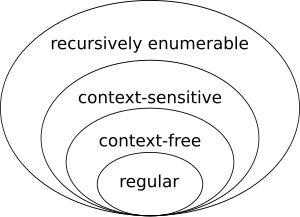
\includegraphics[scale = 0.65]{Chomsky-hierarchy.png}
		
	\end{frame}

	\begin{frame}[fragile]{Clasificación del problema de la palabra.}
		
		\begin{teo}[Animisov--1971]
			Sea $G$ un grupo finitamente generado por $A$. 
			Entonces $\WP{G}{A}$ es regular si y solo si $G$ es finito.
		\end{teo}
		
		\TODO{Agregar dibujito de automáta y decir que es lo mismo que el grafo de Cayley en el caso finito.}

		\begin{alertblock}{Pregunta natural.}
			¿Es posible caracterizar a los grupos cuyo lenguaje del problema de la palabra es independiente de contexto?
		\end{alertblock}
	\end{frame}
	
	\begin{frame}[fragile]{Teorema de Muller-Schupp.}
		
		\[	
			\begin{tikzpicture}{scale = 0.75}
				\path 
				(0,0) node(a) [rectangle,draw] {Grupo fundamental de un grafo de grupos finito}
				(5,-3) node(b) [rectangle,draw] {Treewidth finito}
				(0,-6) node(c) [rectangle,draw] {Independiente de contexto}
				(-5,-3) node (d) [rectangle,draw] {Virtualmente libre};
				\draw   
				(d) edge[<-,line width=1.0pt,"Teorema \ref{teo_karrass_solitar}"] (a) 
				(c) edge[<-,line width=1.0pt,"Teorema \ref{teo_Muller_Schupp}"] (d)
				(b) edge[<-,line width=1.0pt,"Teorema \ref{teo_ic_implica_tw}"] (c)
				(a)  edge[<-,line width=1.0pt,"Teorema \ref{coro_tw_finito_implica_pi1}"] (b);
			\end{tikzpicture}
		\]
	\end{frame}

	\begin{frame}[fragile]{Forma normal de Chomsky.}
		\begin{deff}
			Una gramática $\gramatica$ independiente de contexto está en \emph{forma normal de Chomsky} si las producciones son de este tipo:
			\begin{enumerate}
				\item $A \to BC$ donde $A\in V$ y $B,C \in V \setminus \{ S \}$.
				\item $A \to a$ donde $A \in V, a \in \Sigma$.
				\item $S \to \epsilon$ 
			\end{enumerate}
		\end{deff}
		
		\TODO{Agregar intuición de la longitud de la derivación y su relación con la longitud de la palabra.}
	\end{frame}

	\begin{frame}[fragile]{Un lema para forma normal de Chomsky pt 1.}
		
		\begin{columns}
			
			\begin{column}{0.5\textwidth}
				Sea la gramática $\gramatica$ definida por:
				
					 $V = \{ S,A,B,C,D \}$;

					 $\Sigma = \{ a,b,c \}$;
					 
						
						$P = \begin{cases}
								S \to AB \mid CD \mid a \mid b \mid c \\
								A \to CD \mid a \mid b \mid c	\\
								B \to BB \mid a \mid b \mid c	\\
								C \to AB \mid a \mid b \mid c	\\
								D \to DD \mid a \mid b \mid c
						\end{cases}$
						
				
			\end{column}

			\begin{column}{0.5 \textwidth}
				Podemos derivar la palabra $w = caabccab$ del siguiente modo:
				\begin{align*}
					S &\to AB \to CDB \to CDBB \to^{*} CDab \to \\
					ABDab & \to  AbDab   \to AbDDab  \to CDbDDab   \to\\
					CDbccab & \to CDDbccab \to Caabccab \to caabccab \\
				\end{align*}
			\end{column}
		\end{columns}
	\end{frame}

	
	\begin{frame}{Ejemplo forma normal de Chomsky pt.2}
		Consideremos la subpalabra $u  = aabcc$ de $w = caabccab$.
		Consideremos el \textit{árbol de derivación}.
		\TODO{Agregar dibujito y decir que el nodo tal es el más chico que deriva la subpalabra $u$}. 
		
	\end{frame}

	\begin{frame}[fragile]{Un lema para forma normal de Chomsky pt 2.}
		En general vale el siguiente enunciado.

		\begin{lemma}
			Sea $\gramatica$ una gramática independiente de contexto en forma normal de Chomsky.
			Sea $w \in L(\cG)$ tal que $w = tuv$ con $t,u,v \in \Sigma^{*}$. 
			Si fijamos una derivación $S \to^{*} w$ entonces existe un único vértice en el árbol de derivación con la propiedad de ser el más bajo entre aquellos de los que deriva una subpalabra que da lugar a $u$.
		\end{lemma}

		\TODO{Agregar oralmente detalles sobre "da lugar a $u$".}
	\end{frame}
	
	\begin{frame}[fragile]{Teorema de Muller--Schupp.}
		\TODO{Detallar más cada uno de estos nodos.}
		\[	
			\begin{tikzpicture}{scale = 0.75}
				\path 
				(0,0) node(a) [rectangle,draw] {Grupo fundamental de un grafo de grupos finito}
				(5,-3) node(b) [rectangle,draw] {Treewidth finito}
				(0,-6) node(c) [rectangle,draw] {Independiente de contexto}
				(-5,-3) node (d) [rectangle,draw] {Virtualmente libre};
				\draw   
				(d) edge[<-,line width=1.0pt,"Teorema \ref{teo_karrass_solitar}"] (a) 
				(c) edge[<-,line width=1.0pt,"Teorema \ref{teo_Muller_Schupp}"] (d)
				(b) edge[<-,line width=1.0pt,"Teorema \ref{teo_ic_implica_tw}"] (c)
				(a)  edge[<-,line width=1.0pt,"Teorema \ref{coro_tw_finito_implica_pi1}"] (b);
			\end{tikzpicture}
		\]
	\end{frame}

	\begin{frame}{Descomposición en un árbol y treewidth de un grafo.}
	Sea $\Gamma$ un grafo no dirigido.
	Una \emph{descomposición en un árbol} de $\Gamma$ es un par $(T,f)$ donde
	$T$ es un árbol y $f$ una función 
	\[
	f: V(T) \to \partes{V(\Gamma)}
	\]
	Que cumple las siguientes condiciones:
	\begin{enumerate}
		\item Para todo vértice $v \in V(\Gamma)$ debe existir $t \in V(T)$ tal que $v \in f(t)$. 
		\item Para toda arista $\{v,w\} \in E(\Gamma)$ 
		debe existir $t \in V(T)$ tal que $v,w \in f(t)$.
		\item Si $v \in V(\Gamma)$ es tal que $v \in f(t) \cap f(s)$ luego $v \in f(r)$ para todo $r \in V(T)$ en la geodésica que va desde $s$ a $t$.  
	\end{enumerate}
	\end{frame}
	
	\begin{frame}[fragile]{Descomponiendo el grafo de Cayley en un árbol.}
		\TODO{}
	\end{frame}

	\begin{frame}{Descomponiendo el grafo de Cayley en un árbol (ejemplo).}
		\TODO{AAA}
	\end{frame}	
	
	\begin{frame}[fragile]{Independiente de contexto implica treewidth finito (lemas previos).}
		\TODO{}
	\end{frame}

	\begin{frame}[fragile]{Independiente de contexto implica treewidth finito (pt. 1).}
		\TODO{}
	\end{frame}

	\begin{frame}[fragile]{Independiente de contexto implica treewidth finito (pt. 2).}
		\TODO{}
	\end{frame}

\end{document}